\chapter[Use Cases]{Use Cases}\label{cap:use_cases}
In the present chapter we are going to test the UQMS in three different scenarios, spatial only domain, section \ref{Wave Propagation} , spatio-temporal domain, section \ref{spatio_temporal}, and finally a multidisciplinary system, section \ref{NASA}. 

\section{Case Study:  Wave Propagation Problem}\label{Wave Propagation}
As a first case study we use the “HPC4E Seismic Test Suite”, a collection of four 3D models and sixteen associated tests that can be downloaded freely at the project's website (\url{https://hpc4e.eu/downloads/datasets-and-software}) \cite{deLaPuente2015}. Those models have been designed as a set of 16 layers with constant physical properties. The top layer delineates the topography and the other 15 delineate different layer interface surfaces or horizons. A Matlab script is provided that generates 3D gridded volumes and 2D gridded layer surfaces for any desired spacing and for three different variables $v_{p}(m/s)$, $v_{s}(m/s)$ and $density(Kg/m^3)$. For example, to generate a 3D volume with dimensions $250\times501\times501$ in the $v_{p}(m/s)$ variable we can use the values of Table \ref{tab:valuesOfVp}, and run the Matlab script \textit{generate\_hpc4e\_grid.m}.

\begin{table}[H]
\begin{center}
    \begin{tabular}{|l|l|}
    \hline
    \textbf{Layer} & $v_{p}(m/s)$ \\ \hline
    1     & 1618.92 \\ \hline
    2     & 1684.08 \\ \hline
    3     & 1994.35 \\ \hline
    4     & 2209.71 \\ \hline
    5     & 2305.55 \\ \hline
    6     & 2360.95 \\ \hline
    7     & 2381.95 \\ \hline
    8     & 2223.41 \\ \hline
    9     & 2712.06 \\ \hline
    10    & 2532.22 \\ \hline
    11    & 2841.03 \\ \hline
    12    & 3169.31 \\ \hline
    13    & 3252.35 \\ \hline
    14    & 3642.28 \\ \hline
    15    & 3659.22 \\ \hline
    16    & 4000.00 \\ \hline
    \end{tabular}
    \caption {Values of $v_{p}$ used in the generation of a single velocity field cube.}
    \label{tab:valuesOfVp}
    \end{center}
\end{table}

The first slice of this 3D volume generated by the script is shown in Figure \ref{fig:slice1}.

\begin{figure}[H]
    \centering
    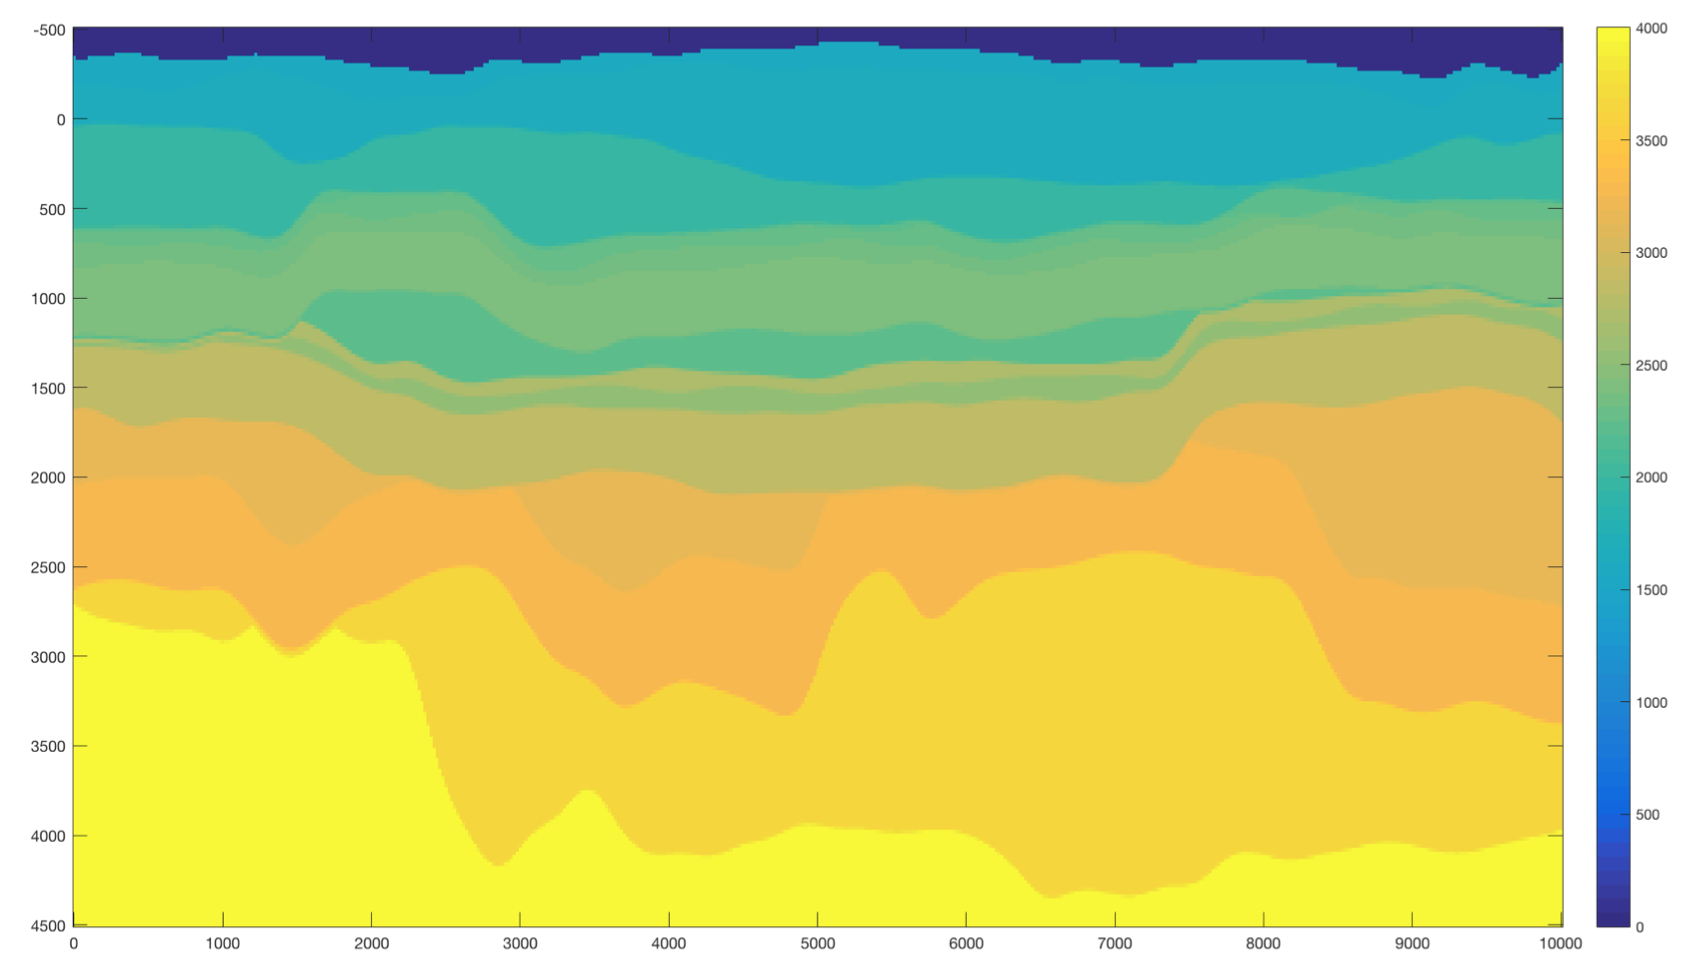
\includegraphics[width=0.8\textwidth]{images/velocity_field.png}
    \caption{One slice of the $250\times501\times501$ cube. In the slice we can distinguish between the different layers.}
    \label{fig:slice1}
\end{figure}

\subsection{The Dataset}
The Matlab script \textit{generate\_hpc4e\_grid.m} could be consider as a mathematical model (black box) $v_{p}(x,y,z) = \mathcal{M}(v_{p})$ that receive $v_{p}$ as an input variable and generate a $v_{p}(x,y,z)$ as an output. In the benchmark the values of $v_{p}$ are fixed (Table \ref{tab:valuesOfVp}), so we cannot use it as is. We need to take the input, $v_{p}(m/s)$  in this case, as a random variable. To achieve this, we designate a \textit{PDFs} to each $v_{p}$ for each layer as shown in Table \ref{tab:PDFsOfVp}.

\begin{table}[H]
\begin{center}
    \begin{tabular}{|l|l|l|}
    \hline
    \textbf{Layer} & \textbf{PDF Family}                & \textbf{Parameters}           \\ \hline
    1     & Gaussian & [1619, 711.2] \\ \hline
    2     & Gaussian & [3368, 711.2]               \\ \hline
    3     & Gaussian & [8839, 711.2]               \\ \hline
    4     & Gaussian & [7698, 301.5]               \\ \hline
    5     & Lognormal   & [7723, 294.7]               \\ \hline
    6     & Lognormal   & [7733, 292.2]               \\ \hline
    7     & Lognormal   & [7658, 312.1]               \\ \hline
    8     & Lognormal   & [3687, 368.7]               \\ \hline
    9     & Exponential & [3949, 394.9]             \\ \hline
    10   & Exponential & [5983, 711.2]               \\ \hline
    11   & Exponential & [3520, 352.0]              \\ \hline
    12   & Exponential & [3155, 315.5]              \\ \hline
    13   & Uniform     & [2541, 396.4]              \\ \hline
    14   & Uniform     & [2931, 435.3]              \\ \hline
    15   & Uniform     & [2948, 437.0]             \\ \hline
    16   & Uniform     & [3289, 471.1]              \\ \hline
    \end{tabular}
    \caption {PDFs and its parameters used to sampling the $v_{p}$, to generate n velocity models.}
    \label{tab:PDFsOfVp}
    \end{center}
\end{table}

Now, using a Monte Carlo method we can sampling the input variable $v_{p}$ and run as many simulations as we want using the model $v_{p}(x,y,z) = \mathcal{M}(v_{p})$, to posteriorly analyze the uncertainty in the output $v_{p}(x,y,z)$. An example of 1000 samplings of $v_{p}$ is shown in Figure \ref{fig:vp_1000_realizations}. Is clear that this is a not a real problem as a benchmark was not conceived as an uncertainty problem, but the datasets generated here are useful for our purposes.

\begin{figure}[ht]
    \centering
    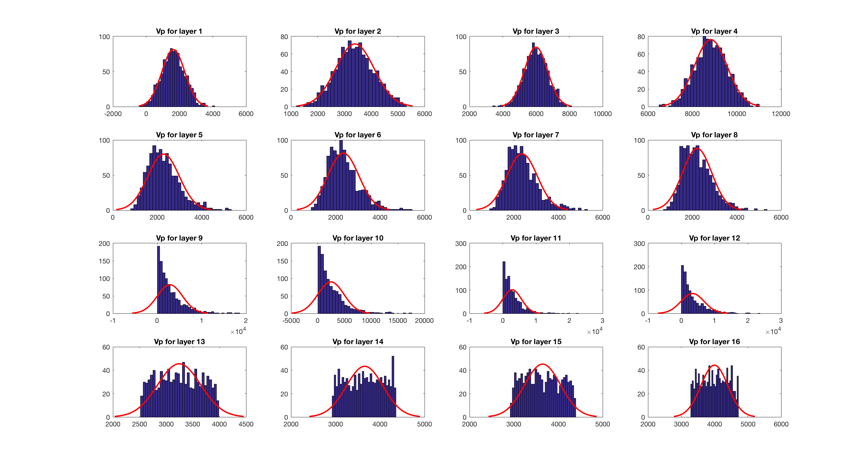
\includegraphics[width=0.8\textwidth]{images/vp_1000_realizations.png}
    \caption{Histograms of the 1000 samplings generated using Monte Carlo method and the PDFs reported in Table \ref{tab:PDFsOfVp}.}
    \label{fig:vp_1000_realizations}
\end{figure}

Using the 1000 samplings of Figure \ref{fig:vp_1000_realizations}, we run the model $v_{p}(x,y,z) = \mathcal{M}(v_{p})$ times, to generate 1000 3D cubes with dimensions of $250\times501\times501$. The full dataset is a multidimensional array of $250\times501\times501\times1000$ with a size og 245 GB. 

To simplify the computational process and visualize the results, we select the slice 200 of each 3D cubes, then our dataset is now a multidimensional array of $250\times501\times1000$. This case study is a the spatial domain only, then the equation \ref{eq:data_base_structure} can be rewrited as $S(x_{i},y_{j},simId,v_{p}(x_{i},y_{j}))$, where $i=1, 2,...,250$, $j=1, 2,...,501$ and $simId = 1, 2,...,1000$. In this new representation $(x_{i},y_{j})$ are the 2D coordinates and $v_{p}(x_{i},y_{j})$ is the velocity value at point $(x_{i},y_{j})$. \textit{simId} still represents the Id of the simulation.

Now that we have an experimental dataset we can apply the proposed workflow step by step.

\subsection{Fitting the GLD}
The first step is to find the \textit{GLD} that best fits the dataset at each spatial location. Running the algorithm proposed in Section \ref{gldFitProcess} we get as a result a new 2D array:
\begin{equation}\label{eq:gld_fit_2D}
S'(x_{i},y_{j},GLD(\lambda_{1}, \lambda_{2}, \lambda_{3}, \lambda_{4}))
\end{equation}
The raw data is reduced and our dataset is characterized by four lambda values at each spatial location. Now we need to assess the validity of the \textit{GLDs} and how well they fit the dataset. Those analyses are described in sections \ref{useCaseGLDValidityCheck} and \ref{useCaseQualityofFit}. 

\subsubsection{GLD validity check}\label{useCaseGLDValidityCheck}
Once the algorithm to check the validity of the \textit{GLD} is run on the experimental dataset, we obtain as a result that the \textit{GLD} is valid in all the $(x_{i},y_{j})$ space.

\subsubsection{Quality of the fit}\label{useCaseQualityofFit}
The next step is to check how good is the fit. To do this we use an algorithm that returns the \textit{D} and \textit{p-value} for the KS-test at each spatial location. As we show in figure \ref{fig:p_value}, and remember that with a \textit{p-value} $>0.05$ we cannot reject the null hypothesis, we conclude that the fit of the GLD is acceptable in most cases. To be more exact, the p-value was greater than 0.05 in 82 \% of the spatial locations, figure \ref{fig:p_values_greater_05}.

\begin{figure}[H]
    \centering
    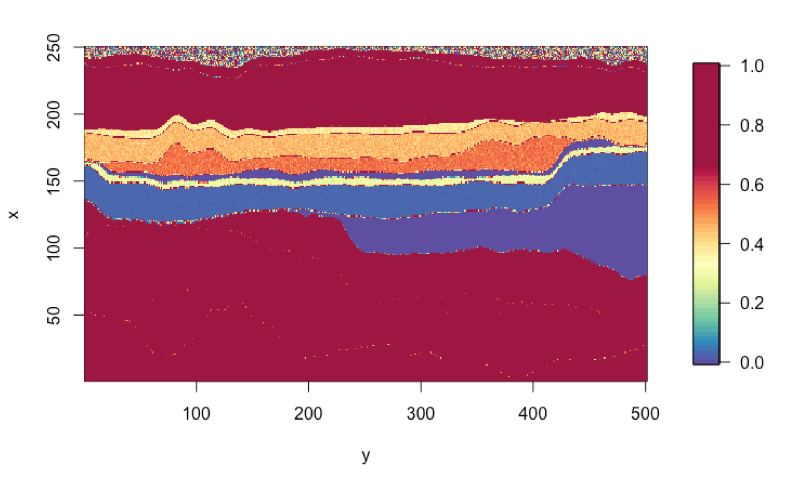
\includegraphics[width=0.8\textwidth]{images/p_value.png}
    \caption{Goodness of the fit based on the \textit{p}-value returning by the KS-test. \textit{p}-value $>$ 0.05 represent a good fit of the GLD to the dataset at $(x_{i}, y_{j})$.}
    \label{fig:p_value}
\end{figure}

\begin{figure}[H]
    \centering
    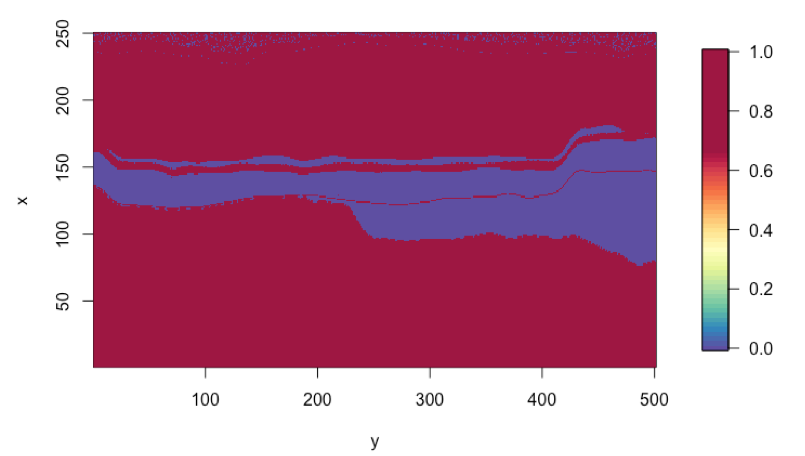
\includegraphics[width=0.8\textwidth]{images/p_value_greater_05.png}
    \caption{The red color shows where the p-value was greater than 0.05.}
    \label{fig:p_values_greater_05}
\end{figure}

If we consider the distance \textit{D}, returned by the KS-test, the result is similar, figure \ref{fig:kolmogorov_distance}. We can see a blue region that is common in figures \ref{fig:p_values_greater_05} and \ref{fig:kolmogorov_distance}. This region is where the quality of the GLD fit is below a threshold. 
%In order to understand what happens in this region, we manually analyze some spatial points inside it. The result is shown in Figure 53. In fact, all the points we analyzed presented the same behavior as the one depicted in Figure 53, modelled as an exponential distribution. Visually, the fit looks good but the KS-test is suggesting a different situation. 
On those cases, some \textit{GLD} extensions proposed in \cite{Karian2011} could be used.

As the main purpose of this thesis is to demonstrate the utility of the use of the \textit{GLD} in \textit{UQ}, then we are not going to deep in other algorithms to solve this particular problem.

\begin{figure}[H]
    \centering
    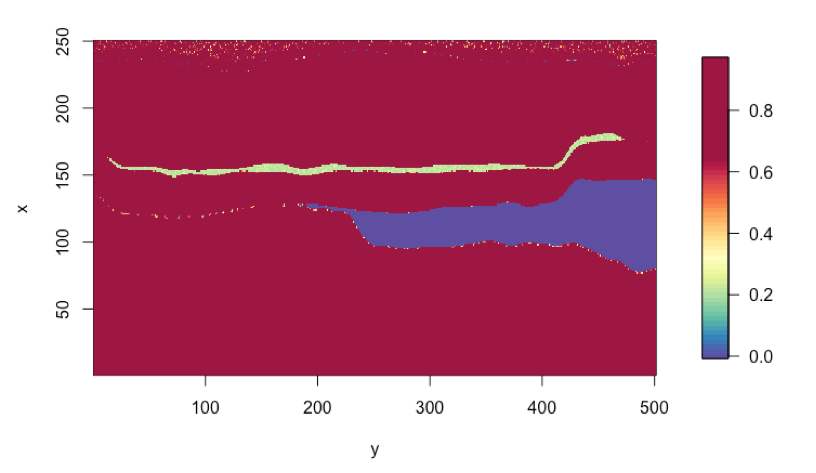
\includegraphics[width=0.8\textwidth]{images/kolmogorov_distance.png}
    \caption{Kolmogorov-Smirnoff Distance (D). The red regions represent where the GLD fits well.}
    \label{fig:kolmogorov_distance}
\end{figure}

\subsection{Clustering}\label{useCaseClustering}
At this point we have our dataset characterized by the $lambda$ values of the \textit{GLDs} on each $(x_{i},y_{j})$, then using the clustering algorithm proposed in Section \ref{sec:clustering}, over $(\lambda_{2}, \lambda_{3}, \lambda_{4})$ values, we get a result shown in Figure \ref{fig:clusters}. A new dataset is produced, where for each spatial location we have a label that indicates the cluster the GLD at each position belongs to (see the schema at Equation \ref{eq:clustersresult}). Note that, in Figure \ref{fig:clusters}, the blue region corresponding to cluster 11 is not a cluster itself. It is rather the region where the \textit{GLD} is not valid, see section \ref{useCaseQualityofFit}.

\begin{equation}\label{eq:clustersresult}
S_{\mathcal{C}}(x_{i},y_{j},clusterID, GLD_{x_{i},y_{j}})
\end{equation}

\begin{figure}[H]
    \centering
    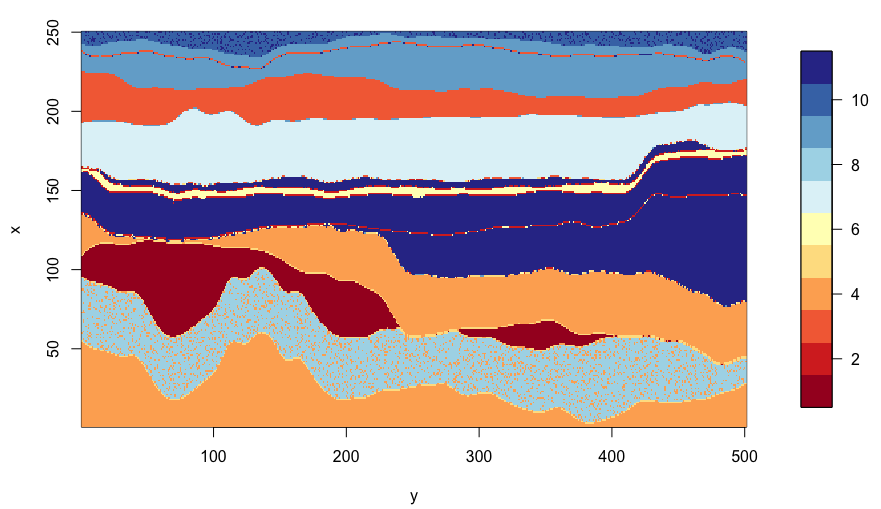
\includegraphics[width=0.8\textwidth]{images/clusters1.png}
    \caption{Result of the clusterization using the clustering algorithm proposed in Section \ref{sec:clustering}, over $(\lambda_{2}, \lambda_{3}, \lambda_{4})$ values with $n=10$.}
    \label{fig:clusters}
\end{figure}

If we compare visually Figures \ref{fig:slice1} and \ref{fig:clusters}, we observe a close similarity. It is clear that they can not be equal because we are talking about a slice of a deterministic model, and the result of clustering 1000 realizations of a stochastic model, but as the model used here is very linear, this is the result we expect.

Another interesting result is shown in Figure \ref{fig:clusters_lambda3_lambda4_space}, where we plot the clusters in $(\lambda_{3}, \lambda_{4})$ space. As we mention in section \ref{sec:gld_shapes}, the shape of the \textit{GLD} depends on the values of $\lambda_{3}$ and $\lambda_{4}$. In this scenario, the expected result is that the members of the same cluster share similar values of $\lambda_{3}$ and $\lambda_{4}$, that is exactly the result we can observe in this figure. 

\begin{figure}[H]
    \centering
    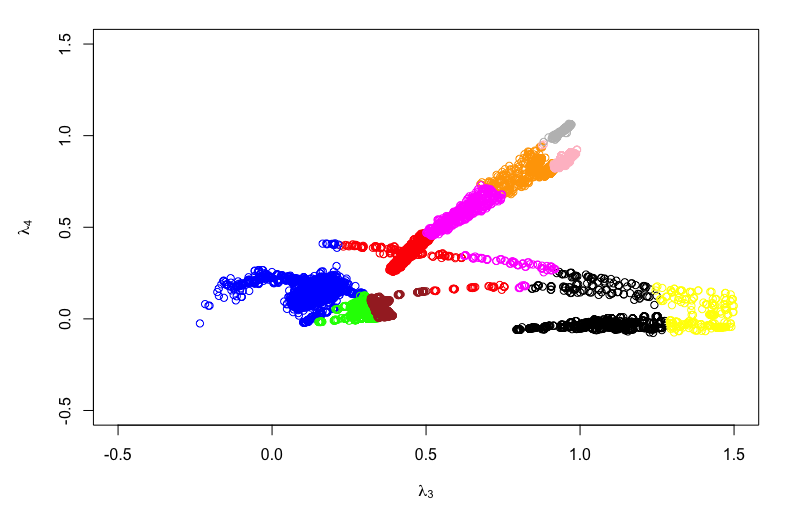
\includegraphics[width=0.8\textwidth]{images/Clusters_lambda3_lambda4.png}
    \caption{Distribution of the clusters in the $(\lambda_{3}, \lambda_{4})$ space. The points that belongs to a same cluster are one near the others, as was expected.}
    \label{fig:clusters_lambda3_lambda4_space}
\end{figure}

To further corroborate this fact, in Figure \ref{fig:cluster1} we show the \textit{PDFs} of 60 members of the 10 clusters. Visually assessing the figures we have an idea of how similar are the shapes of the members of the same cluster and how dissimilar are the shapes of the  members of different clusters. This suggests that our approach is valid. A product of these observations is that we can pick one member of each cluster (the centroid) as a representative of all the members of the cluster, Table \ref{tab:center_of_the_clusters}. The selected member is used to answer the queries in the next sections.

\begin{figure}[H]
    \centering
    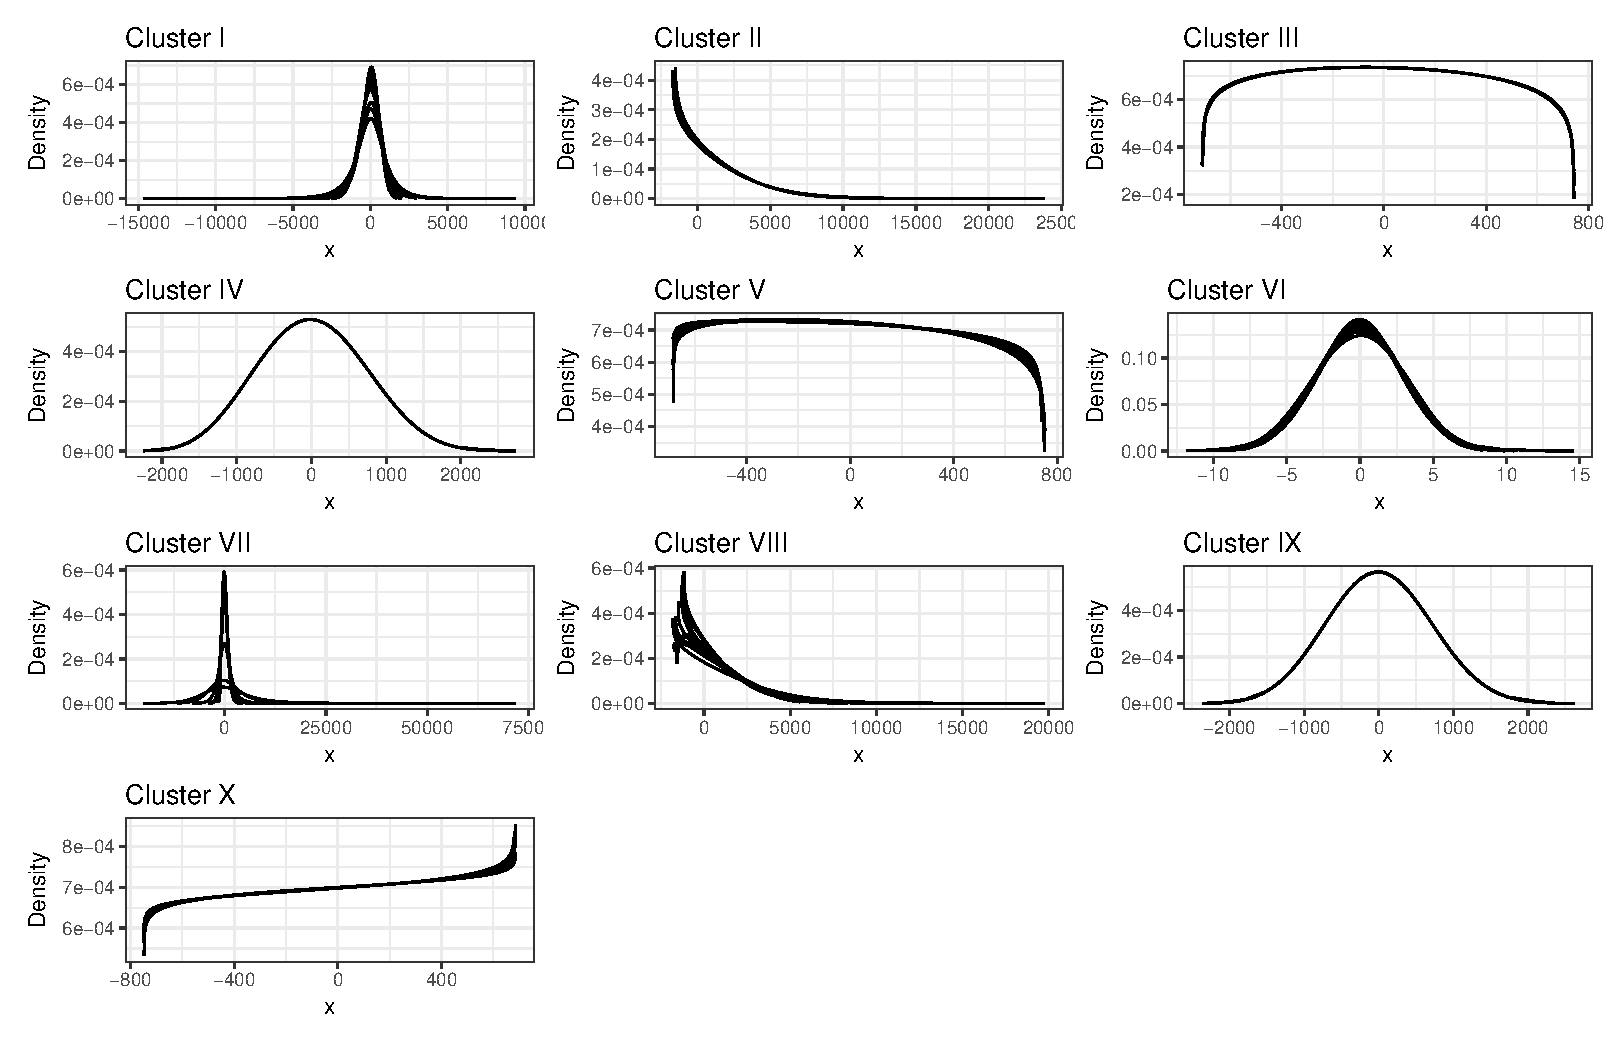
\includegraphics[width=\textwidth]{img/use_cases/clusters.eps}
    \caption{\textit{PDFs} of 60 members of the 10 clusters obtained using the clustering algorithm proposed in Section \ref{sec:clustering}, over $(\lambda_{2}, \lambda_{3}, \lambda_{4})$ values.}
    \label{fig:cluster1}
\end{figure}

\begin{table}[H]
\begin{center}
    \begin{tabular}{|l|l|l|l|}
    \hline
    \textbf{Cluster} & $\lambda_{2}$ & $\lambda_{3}$ & $\lambda_{4}$         \\ \hline
    1     & 0.0013937313 & 0.9585829 & 1.04696461              \\ \hline
    2     & 0.0005291388 & 1.1633978 & -0.07162550            \\ \hline
    3     & 0.0020630696 & 0.1349486 & 0.17305941            \\ \hline
    4     &  0.0016238358 & 0.8653824 & 0.83857646               \\ \hline
    5     & 0.0027346929 & 0.5084664 & 0.39199164                \\ \hline
    6     & 0.0003894541 & 1.4076354 & -0.01925743               \\ \hline
    7     & 0.0021972784 & 0.3253562 & 0.01493809                 \\ \hline
    8     & 0.0015421749 & 0.9491101 & 0.86699555                \\ \hline
    9     & 0.0018672401 & 0.2176002 & 0.17862024            \\ \hline
    10   & 0.4856397733 & 0.1404140 & 0.14011298             \\ \hline
    \end{tabular}
    \caption {Centers of the clusters obtained using the clustering algorithm proposed in Section \ref{sec:clustering}, over $(\lambda_{2}, \lambda_{3}, \lambda_{4})$ values.}
    \label{tab:center_of_the_clusters}
    \end{center}
\end{table}

The 125250 points of the slice are distributed through the clusters following the histogram of the figure \ref{fig:Clusters_histogram} and Table \ref{tab:distribution_of_the_clusters}. 

\begin{figure}[H]
    \centering
    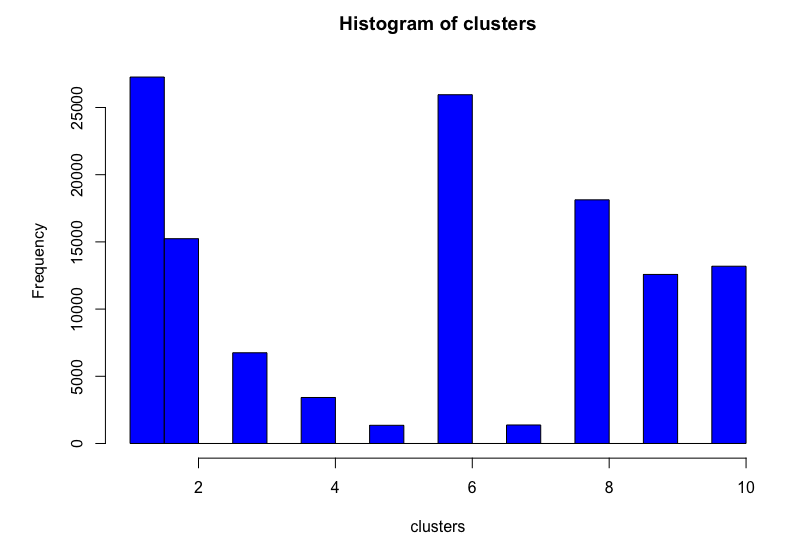
\includegraphics[width=0.8\textwidth]{images/Clusters_histogram.png}
    \caption{Distribution of the clusters.}
    \label{fig:Clusters_histogram}
\end{figure}

\begin{table}
\begin{center}
    \begin{tabular}{|l|l|l|}
    \hline
    \textbf{Cluster} & \textbf{No. of members}         \\ \hline
    1     & 27217              \\ \hline
    2     & 15223             \\ \hline
    3     & 6749            \\ \hline
    4     & 3421               \\ \hline
    5     & 1353                \\ \hline
    6     & 25853               \\ \hline
    7     & 1374                 \\ \hline
    8     & 18103                 \\ \hline
    9     & 12051            \\ \hline
    10   & 13156              \\ \hline
    \end{tabular}
    \caption {Distribution of the clusters.}
    \label{tab:distribution_of_the_clusters}
    \end{center}
\end{table}

\subsection{Spatio-temporal queries}\label{spatio_temporal_queries}
At this point, the initial dataset is summarized as depicted by the schema in equation \ref{eq:clustersresult}. It can be used to answer queries and to validate our approach, comparing the results with the raw data.

First of all we select four spatio-temporal regions of the dataset where the clusters suggest us different behaviors. The regions are shown in Figure \ref{fig:analysis_regions} and the values of $[x_{1}, x_{2}], [y_{1}, y_{2}]$ that define the regions are shown in Table \ref{tab:analysis_regions}. 

\begin{figure}[H]
    \centering
    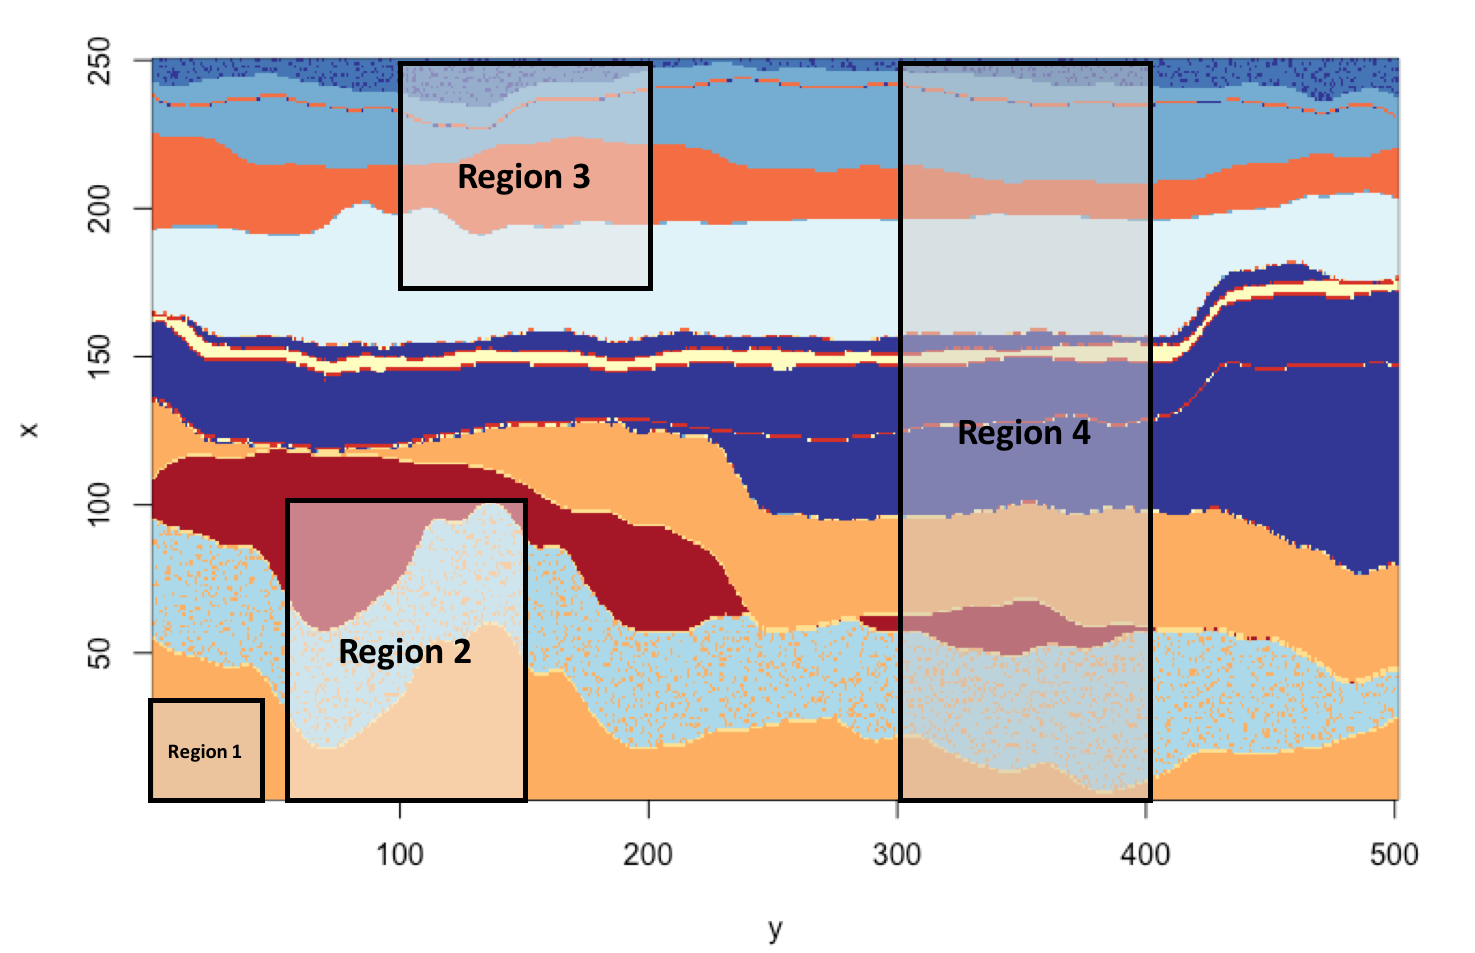
\includegraphics[width=0.8\textwidth]{images/regions.png}
    \caption{Analysis Regions.}
    \label{fig:analysis_regions}
\end{figure}

\begin{table}
\begin{center}
    \begin{tabular}{|l|l|l|l|l|}
    \hline
    \textbf{Region} & $x_{1}$ & $x_{2}$ & $y_{1}$ & $y_{2}$        \\ \hline
    Region 1     & 210 & 250 & 0 & 40              \\ \hline
    Region 2     & 150 & 250 & 50 & 150           \\ \hline
    Region 3     & 0 & 75 & 100 & 200            \\ \hline
    Region 4     & 0 & 250 & 300 & 400               \\ \hline
    \end{tabular}
    \caption {Analysis Regions.}
    \label{tab:analysis_regions}
    \end{center}
\end{table}

With these four regions we assess the adoption of the \textit{GLD} mixture to obtain the \textit{PDF} that characterizes the uncertainty in an specific region, Section \ref{GLDmixtureresults}. In Section \ref{informationEntropyresults} we use the Information Entropy to assign a value that measures the uncertainty at each region. The expected result is that in section \ref{GLDmixtureresults} the GLD mixture characterize correctly the raw data; and in \ref{informationEntropyresults} we expect a zero as a value of the Information Entropy in region 1 and increased values between regions 2, 3 and 4.

\subsubsection{GLD mixture}\label{GLDmixtureresults}
The experiment here is to use the representative \textit{GLDs} at each cluster and the weight associated to it in the region. Using these parameters we can build a \textit{GLD mixture} that characterizes the uncertainty on that region. Here we use the algorithm described in section \ref{sub:gldMixtureWorkflow}.

First of all we query the region to find  the clusters represented inside it, and how are they distributed. Below we show the R codes to query the four regions. The retrieved results are shown in Table \ref{tab:distribution_of_the_clusters_by_regions}.

\begin{equation*}
> clRegion1 = clByRegion(210, 250, 0, 40)
\end{equation*}
\begin{equation*}
> clRegion2 = clByRegion(150, 250, 50, 150)
\end{equation*}
\begin{equation*}
> clRegion3 = clByRegion(0, 75, 100, 200)
\end{equation*}
\begin{equation*}
> clRegion4 = clByRegion(0, 250, 300, 400)
\end{equation*}

\begin{table}[H]
\begin{center}
    \begin{tabular}{|l|l|l|l|l|}
    \hline
    \textbf{Cluster} & \textbf{Region 1} &  \textbf{Region 2} &  \textbf{Region 3} &   \textbf{Region 4}  \\ \hline
    1     & 0   		& 2250 & 0 & 979            \\ \hline
    2     & 0   		& 0 & 0 & 268           \\ \hline
    3     & 0      	& 0 & 2596 & 1468       \\ \hline
    4     & 1640	& 4467 & 0 & 5173         \\ \hline
    5     & 0       & 149 & 0 & 269          \\ \hline
    6     & 0     & 0 & 0 & 416           \\ \hline
    7     & 0       & 0 & 1967 & 3920           \\ \hline
    8     & 0     & 3335 & 0 & 3432             \\ \hline
    9     & 0      & 0 & 1918 & 3280       \\ \hline
    10   & 0      & 0 & 901 & 583         \\ \hline
    \end{tabular}
    \caption {Distribution of the clusters by regions.}
    \label{tab:distribution_of_the_clusters_by_regions}
    \end{center}
\end{table}

If we divide the columns of Table \ref{tab:distribution_of_the_clusters_by_regions} by the sum of the elements of each column we get the weight needed to formulate the \textit{mixed GLDs}. It is clear that the \textit{GLD} in region 1 is represented by the \textit{GLD} of cluster 4. On the other 3 cases we get:

\begin{equation*}\label{eq:pareto mle2}
  \begin{aligned}
& GLD_{region1} = GLD_{c4} \\
& GLD_{region2} = 0.22GLD_{c1} + 0.44GLD_{c4} + 0.014GLD_{c5} \\
& + 0.33GLD_{c8} \\
& GLD_{region3} = 0.34GLD_{c3} + 0.26GLD_{c7} + 0.25GLD_{c9} \\
& + 0.12GLD_{c10} \\
& GLD_{region4} = 0.22GLD_{c1} + 0.44GLD_{c4} + 0.014GLD_{c5} \\ 
& + 0.33GLD_{c8}
\end{aligned}
\end{equation*}

Now we need to evaluate if the \textit{mixture of GLDs} describes well the uncertainty in the regions. To do this we perform the same \textit{ks-test} used to evaluate the goodness of the fit and described in Section \ref{Quality of the fit}. 

\begin{table}[H]
\begin{center}
    \begin{tabular}{|l|l|l|l|l|}
    \hline
    \textbf{Metrics} & \textbf{Region 1} &  \textbf{Region 2} &  \textbf{Region 3} &   \textbf{Region 4}  \\ \hline
    p-value     & 0.73   		& 0.56 & 0.34 & 0.08            \\ \hline
    \end{tabular}
    \caption {p-values by regions.}
    \label{tab:p_values_by_regions}
    \end{center}
\end{table}

Based on the \textit{p-value}, Table \ref{tab:p_values_by_regions}, we can conclude that in all 4 regions the \textit{mixture of GLDs} is a good fit to the raw data.

\subsubsection{Information Entropy}\label{informationEntropyresults}
Now we are going to evaluate what happens with the information entropy. Based on the distribution of clusters inside the regions, table \ref{tab:distribution_of_the_clusters_by_regions}; we can compute the entropy. In this case we use an R function called \textit{entropy}, implemented in the r-package of the same name  \cite{Hausser2008}.

\begin{table}[H]
\begin{center}
    \begin{tabular}{|l|l|l|l|l|}
    \hline
    \textbf{entropy} & \textbf{Region 1} &  \textbf{Region 2} &  \textbf{Region 3} &   \textbf{Region 4}  \\ \hline
    value     & 0   		& 1.122243 & 1.41166 & 2.024246            \\ \hline
    \end{tabular}
    \caption {Information Entropy by regions.}
    \label{tab:entropy_by_regions}
    \end{center}
\end{table}

As we expect, Table \ref{tab:entropy_by_regions}, the entropy in region 1 is zero, because the region contains only members of the cluster 4. On the other regions the entropy increases from region 2 to region 4, as we expected.

It is clear that the information entropy is a very good and simple measure of the uncertainty, and here it is demonstrated its utility combined with the \textit{GLD}.


\section{Case study with cross-correlated variables}
As a second case study we select an example included in an R package \textbf{spus} \cite{Sawicka2016}. This package implement a methodology for uncertainty propagation analysis in spatial environmental. The \textbf{spus} package includes functions for uncertainty model specification, propagation of uncertainty using Monte Carlo (MC) techniques, and uncertainty visualization functions.
The case study describe the spatial distribution of organic carbon (OC) and nitrogen (N), variables that are used to derive $C/N$ ratio, vital information to evaluate soil management and to increase the crop productivity. Maps of OC and N are approximations encumbered with errors. These errors will propagate through the calculation into the $C/N$ prediction.

\subsection{The Dataset}
The example data for $C/N$ calculations are a 250m resolution mean OC and TN (total N) of a $33km \times 33km$ area adjacent to lake Alaotra in Madagascar.

The Madagascar dataset contains four spatial objects: a mean OC and TN of the area and their standard deviations. It also has a saved function that calculates $C/N$ using OC and TN that will be used later.

In Figure \ref{fig:mean_oc_tn} we present the mean of OC and TN in the area.

\begin{figure}[H]
    \centering
    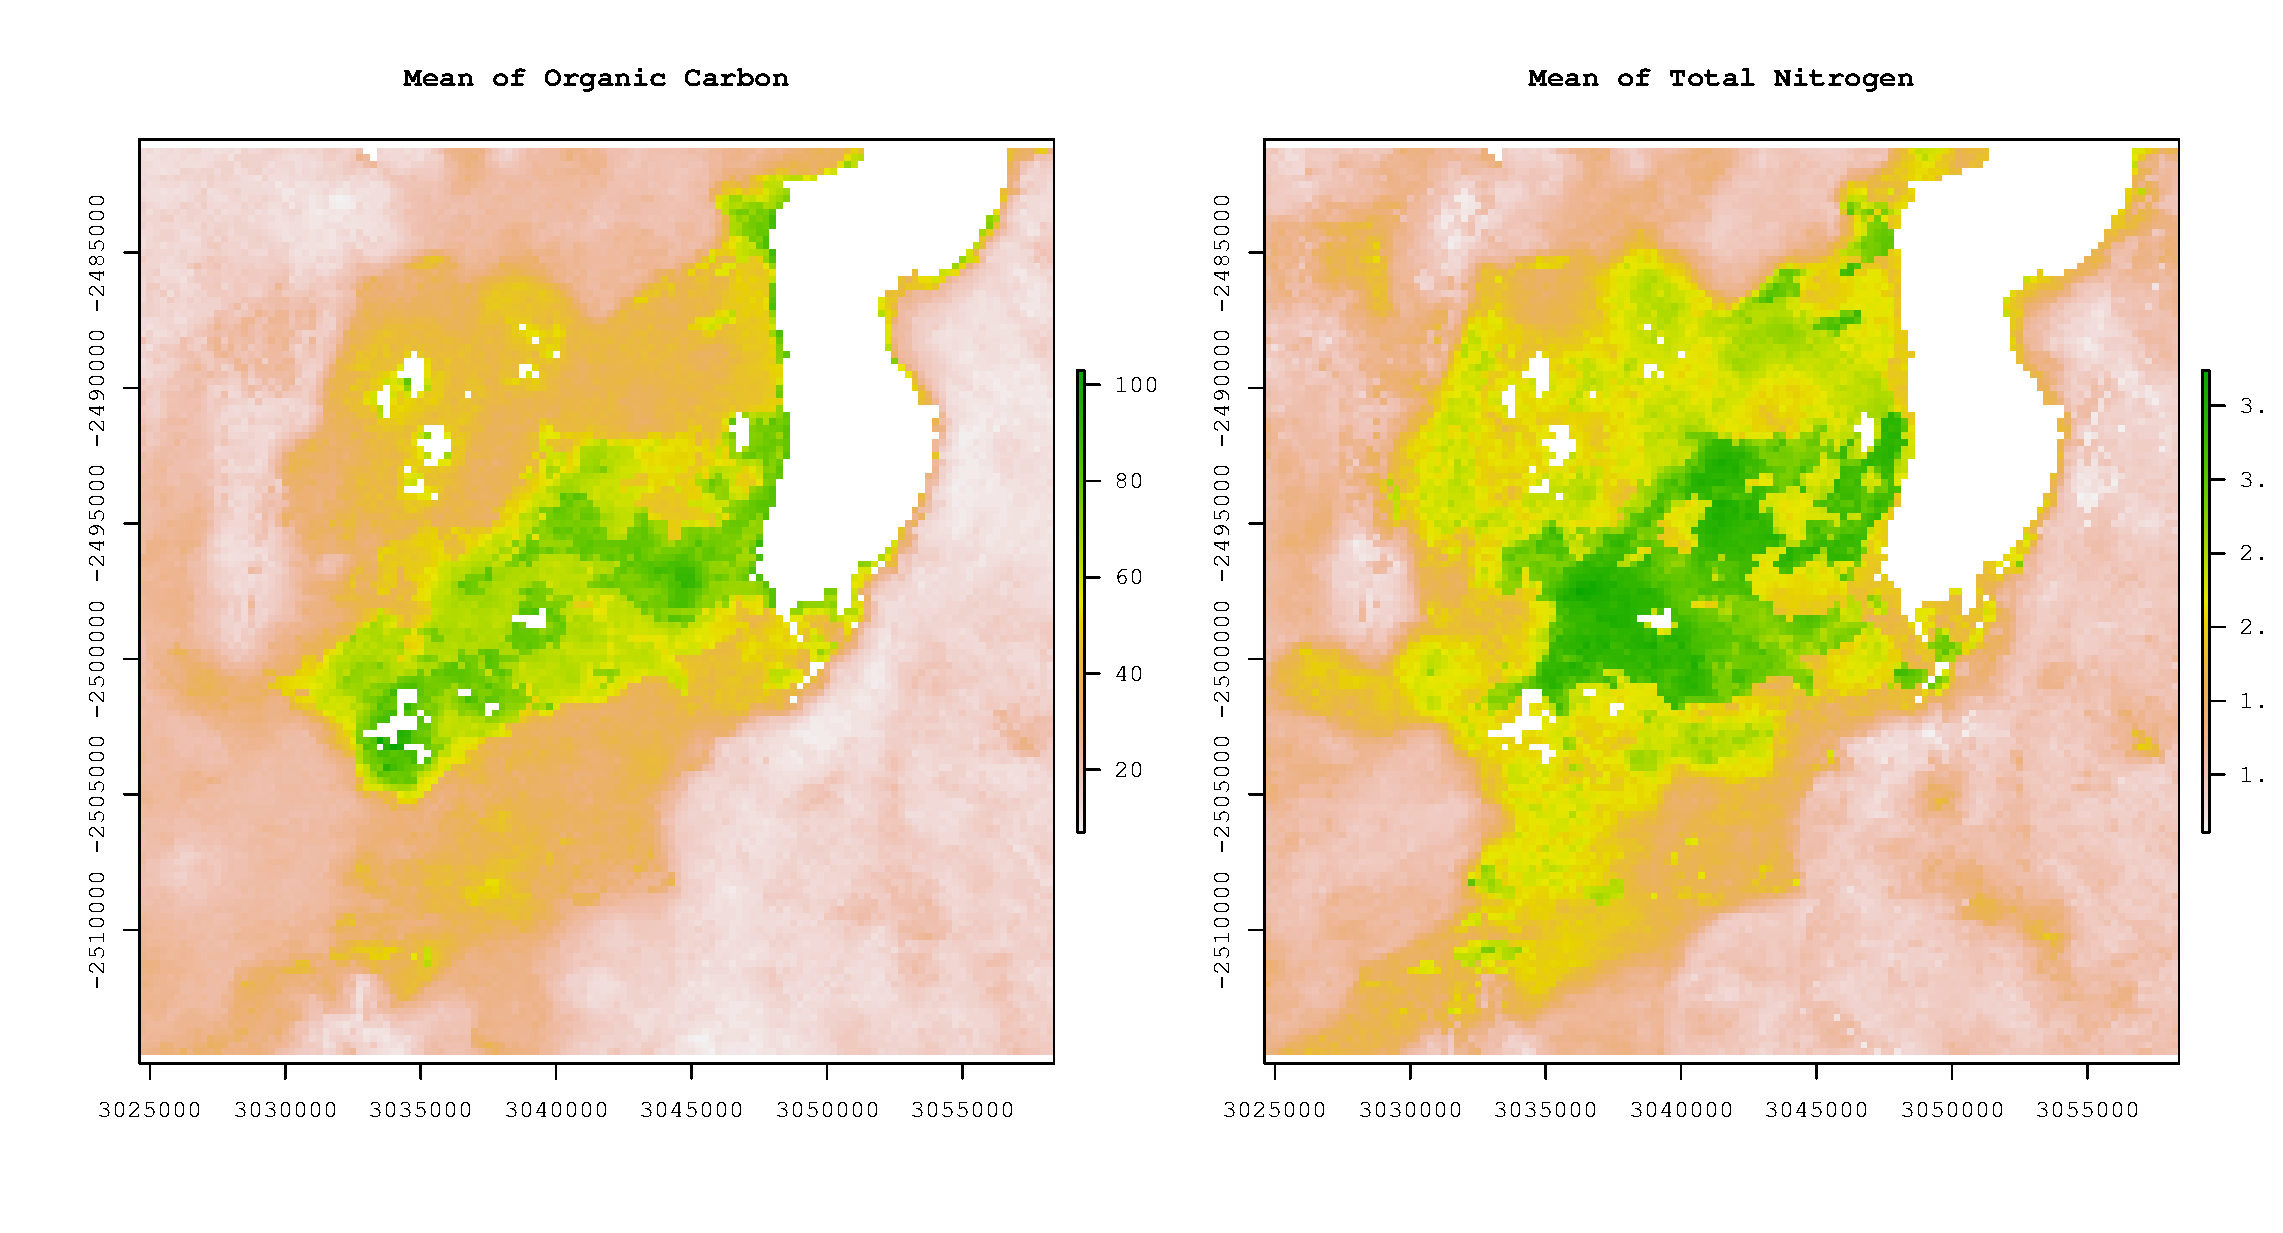
\includegraphics[width=0.8\textwidth]{img/use_cases/spus/dataset_example.eps}
    \caption{Mean of organic carbon (OC) and total nitrogen (TN) of a $33km \times 33km$ area adjacent to lake Alaotra in Madagascar.}
    \label{fig:mean_oc_tn}
\end{figure}

OC and TN are the input variables of a model $C/N = \mathcal{M}(OC, TN)$ defined by an R function as follow:

\begin{lstlisting}[language=R]
function (OC, TN) 
{
    OC/TN
}
\end{lstlisting}

This R function receive OC and TN as inputs and return the $C/N$ ratio. The original Madagascar dataset as it, only contain information about the mean and standard deviation of OC and TN. To propagate the uncertainty through a model, the authors of \textbf{spus} package define OC and TN as uncertain variables. In both cases the uncertainty is characterized by a normal distribution with mean OC and TN and standard deviation OC\_sd and TN\_sd respectively. Using a Monte Carlo method, the author sampling the input space to obtain 500 realizations. 

The propagation of uncertainty occurs when the model is run with the uncertain inputs. Running the model with a sample of realizations of uncertain input variable(s) yields an equally large sample of model outputs that can be further analyzed, in this case 500 samples of $134 \times 135$.

\subsection{Fitting the GLD}
Now that we have the output dataset, lets proceed to use our approach. The first step is the fitting process, find the \textit{GLD} that best fit the dataset on each location. Similar to the previous use case, we use the fitting functions of the \textbf{suq$^2$} package. In all the spatial locations the algorithm return a valid \textit{GLD} with $p_{value} > 0.05$. 

\subsection{Queries}
The main question the researchers of the \textbf{spus} package are interesting in is identify all locations where the $C/N$ ratio is smaller than 24, with 90\% probability. This information might be used by farmers to identify which plots require action on improving soil quality.

This question is not part of the queries we propose in our approach. So, we show now, how queries like this one are simple to answer with our approach, demonstrating how easy is to extend it.

The \textit{GLD} is defined by it quantile function (see Section \ref{sec:parameterizations}). The question of \textit{"locations where the $C/N$ ratio is smaller than 24, with 90\% probability"} can be translated as: \textit{"locations where the 90\% percentile of the distribution is less or equal to 24"}. 

To answer this question two new algorithms are proposed (could be one algorithm but to warranty that the functions are sufficiently generic, we propose a two algorithms), Algorithm \ref{alg:quantileValueGLD} to compute the value of the quantile $q$ of the \textit{GLD} over a spatio-temporal region $(s_{i},t_{j})$, and Algorithm \ref{alg:quantileValue2GLD} to compare if the quantile value returned by the previous algorithm is less or equal to the desired value.

\begin{algorithm} 
\caption{This Algorithm return the value of the quantile $q$ for each \textit{GLD} in $(s_{i},t_{j})$.}\label{alg:quantileValueGLD}
\begin{algorithmic}[1] 
\Function{gldQuantile}{$S(s_{i},t_{j}, <\lambda_{1},\lambda_{2},\lambda_{3},\lambda_{4}>), q$} 
\For{\textbf{each} $(s_{i},t_{j})$}
\State $S(s_{i},t_{j}, q_{value}) \gets \Call {suq2.utils.qgl}{S(s_{i},t_{j}, <\lambda_{1},\lambda_{2},\lambda_{3},\lambda_{4}>), q}$
\EndFor
\EndFunction 
\end{algorithmic} 
\end{algorithm} 

\begin{algorithm} 
\caption{This Algorithm assigns a 1 to $S(s_{i},t_{j}, q_{result})$ if the value at this position meets the condition, and 0 otherwise.}\label{alg:quantileValue2GLD}
\begin{algorithmic}[1] 
\Function{gldQuantileCompare}{$S(s_{i},t_{j}, q_{value}), q_{compare}$} 
\For{\textbf{each} $(s_{i},t_{j})$}
\If{$q_{value} \leq q_{compare}$}
\State $S(s_{i},t_{j}, q_{result}) \gets 1$
\Else
\State $S(s_{i},t_{j}, q_{result}) \gets 0$
\EndIf
\EndFor
\EndFunction 
\end{algorithmic} 
\end{algorithm} 

In lines 4 and 6 of Algorithm \ref{alg:quantileValue2GLD} we assign a value 1 or 0 if the quantile at position $(s_{i},t_{j})$ meets the condition or not. Figures \ref{fig:resp_spus} and \ref{fig:resp_suq2} show the resultant images of the \textbf{spus} and \textbf{suq$^2$} respectively. The results is not exactly the same as we can see by simple observation, but is extremely similar. To be more precise, the comparison of both image matrix return a 89\% of similarity.

\begin{figure}[H]
    \centering
    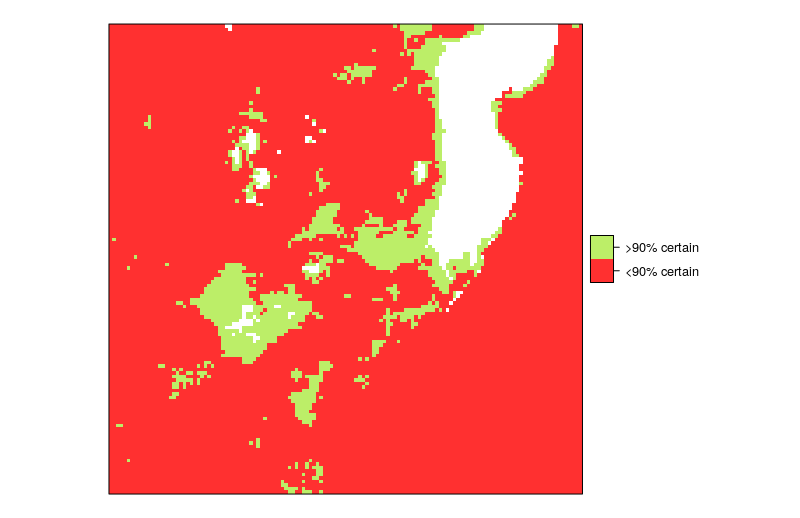
\includegraphics[width=0.8\textwidth]{img/use_cases/spus/respuesta_spus2.png}
    \caption{Locations where the $C/N$ ratio is smaller than 24, with 90\% probability, \textbf{spus} package.}
    \label{fig:resp_spus}
\end{figure}

\begin{figure}[H]
    \centering
    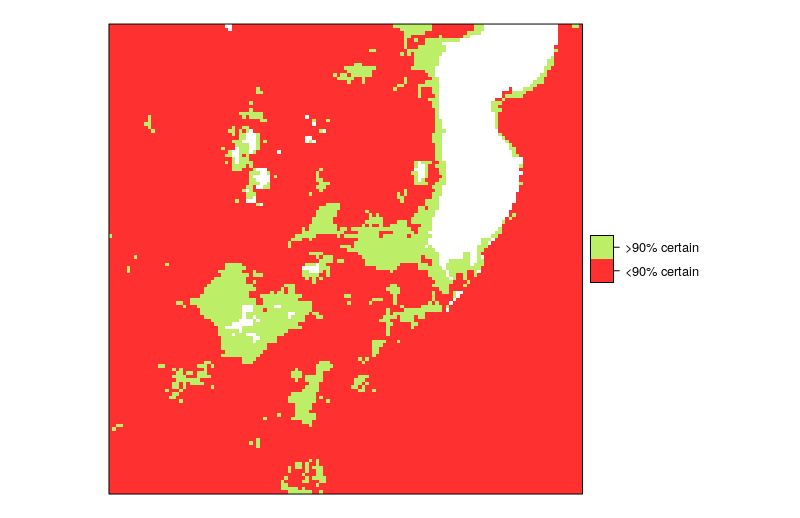
\includegraphics[width=0.8\textwidth]{img/use_cases/spus/respuesta_suq22.png}
    \caption{Locations where the $C/N$ ratio is smaller than 24, with 90\% probability, \textbf{suq$^2$} package.}
    \label{fig:resp_suq2}
\end{figure}

\subsection{Clustering}
Although the main objective of this case study was accomplished, we test the proposed workflow with the current dataset. The clustering algorithm was running with



\section{Case Study: Austin, queso library}\label{spatio_temporal}

\section{Case Study: Multidisciplinary System (NASA)}\label{NASA}

\section{Case Study: Spatio-temporal Nicholson-Bailey model}
Este esta en el software uqlab, en la carpeta Doc Manuals

\section{Summary}\label{sec:use_case_summary}
